\section{Discriminant analysis}
\frame{\sectionpage}



\begin{frame}[fragile]{Discriminant analysis}

  \begin{itemize}
  \item ANOVA and MANOVA: predict a (counted/measured) response from group membership.
  \item Discriminant analysis: predict group membership based on counted/measured variables.
  \item Covers same ground as logistic regression (and its variations), but emphasis on classifying observed data into correct groups.
  \item Does so by searching for linear combination of original variables that best separates data into groups (canonical variables).
  \item Assumption here that groups are known (for data we have). If trying to ``best separate'' data into unknown groups, see {\em cluster analysis}.
  \item Examples: revisit seed yield and weight data, peanut data,
    professions/activities data; remote-sensing data.
  \end{itemize}

\end{frame}


\begin{frame}[fragile]{Packages}
\begin{knitrout}
\definecolor{shadecolor}{rgb}{0.969, 0.969, 0.969}\color{fgcolor}\begin{kframe}
\begin{alltt}
\hlkwd{library}\hlstd{(tidyverse)}
\end{alltt}


{\ttfamily\noindent\itshape\color{messagecolor}{\#\# Loading tidyverse: ggplot2\\\#\# Loading tidyverse: tibble\\\#\# Loading tidyverse: tidyr\\\#\# Loading tidyverse: readr\\\#\# Loading tidyverse: purrr\\\#\# Loading tidyverse: dplyr}}

{\ttfamily\noindent\itshape\color{messagecolor}{\#\# Conflicts with tidy packages ----------------------------------------------}}

{\ttfamily\noindent\itshape\color{messagecolor}{\#\# filter(): dplyr, stats\\\#\# lag():\ \ \ \ dplyr, stats}}\begin{alltt}
\hlkwd{library}\hlstd{(ggrepel)}
\end{alltt}
\end{kframe}
\end{knitrout}

\texttt{ggrepel} allows labelling points on a plot so they don't
overwrite each other.
\end{frame}

\begin{frame}[fragile]{Example 1: seed yields and weights}



  {\small
\begin{minipage}[t]{0.55\linewidth}
\begin{knitrout}
\definecolor{shadecolor}{rgb}{0.969, 0.969, 0.969}\color{fgcolor}\begin{kframe}
\begin{alltt}
\hlstd{hilo}\hlkwb{=}\hlkwd{read.table}\hlstd{(}\hlstr{"manova1.txt"}\hlstd{,}\hlkwc{header}\hlstd{=T)}
\hlkwd{ggplot}\hlstd{(hilo,}\hlkwd{aes}\hlstd{(}\hlkwc{x}\hlstd{=yield,}\hlkwc{y}\hlstd{=weight,}\hlkwc{colour}\hlstd{=fertilizer))}\hlopt{+}
  \hlkwd{geom_point}\hlstd{(}\hlkwc{size}\hlstd{=}\hlnum{4}\hlstd{)}
\end{alltt}
\end{kframe}
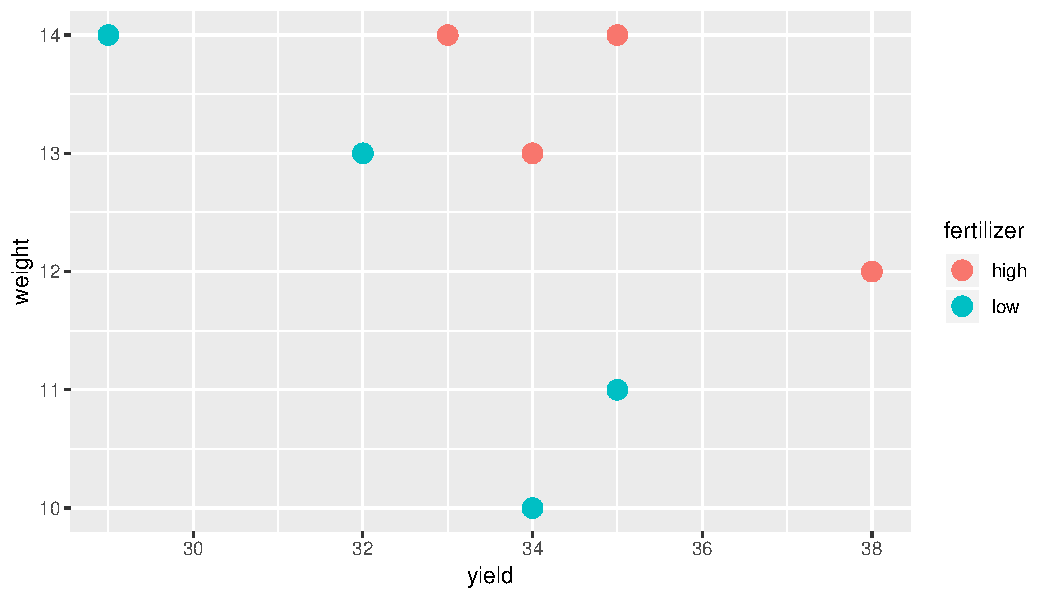
\includegraphics[width=\maxwidth]{figure/berzani-1} 

\end{knitrout}
\end{minipage}
}
\begin{minipage}[t]{0.37\linewidth}
  \vspace{1in}
  Recall data from MANOVA: needed a multivariate analysis to find
  difference in seed yield and weight based on whether they were high
  or low fertilizer.
  
\end{minipage}

  
\end{frame}



\begin{frame}[fragile]{Basic discriminant analysis}

\begin{knitrout}
\definecolor{shadecolor}{rgb}{0.969, 0.969, 0.969}\color{fgcolor}\begin{kframe}
\begin{alltt}
\hlkwd{suppressMessages}\hlstd{(}\hlkwd{library}\hlstd{(MASS))}
\hlstd{hilo.lda}\hlkwb{=}\hlkwd{lda}\hlstd{(fertilizer}\hlopt{~}\hlstd{yield}\hlopt{+}\hlstd{weight,}\hlkwc{data}\hlstd{=hilo)}
\end{alltt}
\end{kframe}
\end{knitrout}

\begin{itemize}
\item Uses \texttt{lda} from package MASS.
\item ``Predicting'' group membership from measured variables.
\end{itemize}

\end{frame}

\begin{frame}[fragile]{Output}

  
  \begin{minipage}[t]{0.6\linewidth}
{\small
\begin{knitrout}
\definecolor{shadecolor}{rgb}{0.969, 0.969, 0.969}\color{fgcolor}\begin{kframe}
\begin{alltt}
\hlstd{hilo.lda}
\end{alltt}
\begin{verbatim}
## Call:
## lda(fertilizer ~ yield + weight, data = hilo)
## 
## Prior probabilities of groups:
## high  low 
##  0.5  0.5 
## 
## Group means:
##      yield weight
## high  35.0  13.25
## low   32.5  12.00
## 
## Coefficients of linear discriminants:
##               LD1
## yield  -0.7666761
## weight -1.2513563
\end{verbatim}
\end{kframe}
\end{knitrout}

}
    
  \end{minipage}
  \begin{minipage}[t]{0.37\linewidth}
  \begin{itemize}
  \item Means on both variables slightly higher for \texttt{high}
    fertilizer.
  \item ``Coefficients of linear discriminant'' say how groups can be
    best separated by original variables.
  \item \textbf{discriminant score} \texttt{LD1} negative when both
    \texttt{yield} and \texttt{weight} high (as $z$-scores), positive
    when both low. 
  \end{itemize}
  \end{minipage}

\end{frame}


\begin{frame}[fragile]{Predictions and predicted groups}
  
\ldots based on \texttt{yield} and \texttt{weight}:

{\footnotesize
\begin{knitrout}
\definecolor{shadecolor}{rgb}{0.969, 0.969, 0.969}\color{fgcolor}\begin{kframe}
\begin{alltt}
\hlstd{hilo.pred}\hlkwb{=}\hlkwd{predict}\hlstd{(hilo.lda)}
\hlkwd{cbind}\hlstd{(hilo,}\hlkwc{predicted}\hlstd{=hilo.pred}\hlopt{$}\hlstd{class)}
\end{alltt}
\begin{verbatim}
##   fertilizer yield weight predicted
## 1        low    34     10       low
## 2        low    29     14       low
## 3        low    35     11       low
## 4        low    32     13       low
## 5       high    33     14      high
## 6       high    38     12      high
## 7       high    34     13      high
## 8       high    35     14      high
\end{verbatim}
\begin{alltt}
\hlkwd{table}\hlstd{(}\hlkwc{observed}\hlstd{=hilo}\hlopt{$}\hlstd{fertilizer,}\hlkwc{predicted}\hlstd{=hilo.pred}\hlopt{$}\hlstd{class)}
\end{alltt}
\begin{verbatim}
##         predicted
## observed high low
##     high    4   0
##     low     0   4
\end{verbatim}
\end{kframe}
\end{knitrout}
}

 
\end{frame}

\begin{frame}[fragile]{Posterior probabilities}
  
  show how clear-cut the classification decisions were:
  
\begin{knitrout}
\definecolor{shadecolor}{rgb}{0.969, 0.969, 0.969}\color{fgcolor}\begin{kframe}
\begin{alltt}
\hlstd{pp}\hlkwb{=}\hlkwd{round}\hlstd{(hilo.pred}\hlopt{$}\hlstd{posterior,}\hlnum{4}\hlstd{)}
\hlstd{d}\hlkwb{=}\hlkwd{data.frame}\hlstd{(hilo,hilo.pred}\hlopt{$}\hlstd{x,pp)}
\hlstd{d}
\end{alltt}
\begin{verbatim}
##   fertilizer yield weight        LD1   high    low
## 1        low    34     10  3.0931414 0.0000 1.0000
## 2        low    29     14  1.9210963 0.0012 0.9988
## 3        low    35     11  1.0751090 0.0232 0.9768
## 4        low    32     13  0.8724245 0.0458 0.9542
## 5       high    33     14 -1.1456079 0.9818 0.0182
## 6       high    38     12 -2.4762756 0.9998 0.0002
## 7       high    34     13 -0.6609276 0.9089 0.0911
## 8       high    35     14 -2.6789600 0.9999 0.0001
\end{verbatim}
\end{kframe}
\end{knitrout}
%$
Only obs.\ 7 has any doubt: \texttt{yield} low for a high-fertilizer,
but high \texttt{weight} makes up for it.
  
\end{frame}

\begin{frame}[fragile]{Revisiting the plot}
  
This data frame containing predictions gives what we need for a plot:

\begin{knitrout}
\definecolor{shadecolor}{rgb}{0.969, 0.969, 0.969}\color{fgcolor}\begin{kframe}
\begin{alltt}
\hlkwd{ggplot}\hlstd{(d,}\hlkwd{aes}\hlstd{(}\hlkwc{x}\hlstd{=fertilizer,}\hlkwc{y}\hlstd{=LD1))}\hlopt{+}\hlkwd{geom_point}\hlstd{()}
\end{alltt}
\end{kframe}
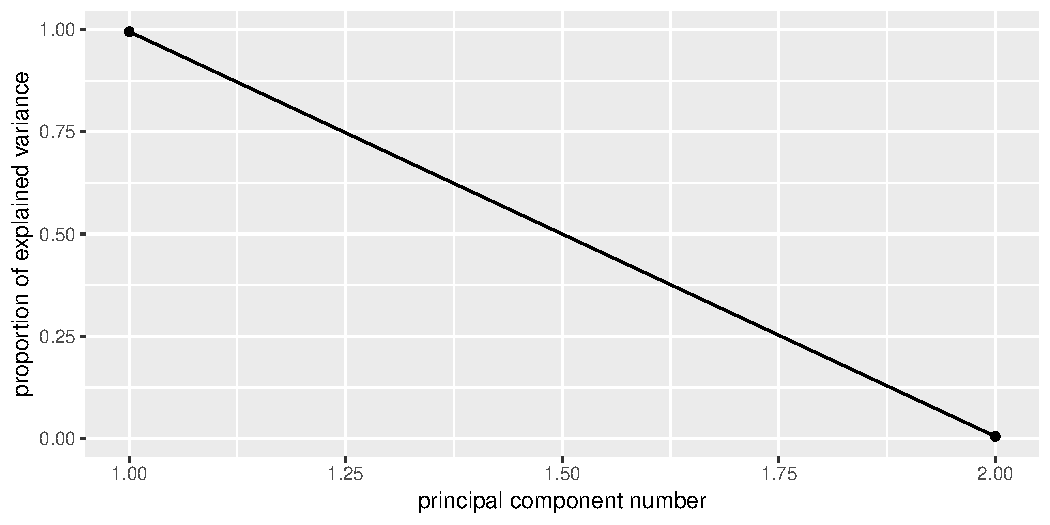
\includegraphics[width=\maxwidth]{figure/unnamed-chunk-7-1} 

\end{knitrout}

\begin{itemize}
\item As before, high and low fertilizer are very distinct on LD1.
\item With more than one \texttt{LD}, plot them against each other.
\end{itemize}
  
\end{frame}



% 
%\begin{frame}[fragile]{Contour plot of \texttt{LD1}}
%
%First, get some new yield and weight values for prediction. Then
%predict \texttt{LD1} for them:
%  
%<<>>=
%yy=seq(29,38,0.5)
%ww=seq(10,14,0.5)
%hilo.new=expand.grid(yield=yy,weight=ww)
%hilo.pred=predict(hilo.lda,hilo.new)
%@ 
%
%Then: plot original data, and overlay contours showing value of
%\texttt{LD1} for each \texttt{yield} and \texttt{weight} (over):
%  
%\end{frame}
%
%\begin{frame}[fragile]{Contour plot}
%
%  \begin{minipage}[t]{0.7\linewidth}
%    
%<<santini,fig.height=5>>=
%plot(yield,weight,col=fno,pch=fno)
%z=matrix(hilo.pred$x,length(yy),
%  length(ww),byrow=F)
%contour(yy,ww,z,add=T)
%@   
%  \end{minipage}
%  \begin{minipage}[t]{0.25\linewidth}
%    \begin{itemize}
%    \item \texttt{LD1} $<0$: top right
%    \item \texttt{LD1} $>0$: bottom left
%    \item \texttt{LD1=0}: boundary between high and low
%    \end{itemize}
%  \end{minipage}
%  
%<<echo=FALSE>>=
%detach(hilo)
%@   
%  
%\end{frame}

\begin{frame}[fragile]{Example 2: the peanuts}

\begin{knitrout}
\definecolor{shadecolor}{rgb}{0.969, 0.969, 0.969}\color{fgcolor}\begin{kframe}
\begin{alltt}
\hlstd{peanuts}\hlkwb{=}\hlkwd{read.table}\hlstd{(}\hlstr{"peanuts.txt"}\hlstd{,}\hlkwc{header}\hlstd{=T)}
\hlkwd{head}\hlstd{(peanuts)}
\end{alltt}
\begin{verbatim}
##   obs location variety     y   smk    w
## 1   1        1       5 195.3 153.1 51.4
## 2   2        1       5 194.3 167.7 53.7
## 3   3        2       5 189.7 139.5 55.5
## 4   4        2       5 180.4 121.1 44.4
## 5   5        1       6 203.0 156.8 49.8
## 6   6        1       6 195.9 166.0 45.8
\end{verbatim}
\end{kframe}
\end{knitrout}

Recall: \texttt{location} and \texttt{variety} both significant in
MANOVA. Make combo of them, separated by \texttt{-} (over):

  
\end{frame}

\begin{frame}[fragile]{Location-variety combos}
  
\begin{knitrout}
\definecolor{shadecolor}{rgb}{0.969, 0.969, 0.969}\color{fgcolor}\begin{kframe}
\begin{alltt}
\hlstd{combo}\hlkwb{=}\hlkwd{with}\hlstd{(peanuts,}\hlkwd{paste}\hlstd{(variety,location,}\hlkwc{sep}\hlstd{=}\hlstr{"-"}\hlstd{))}
\hlstd{combo}\hlkwb{=}\hlkwd{factor}\hlstd{(combo)}
\hlstd{combo}
\end{alltt}
\begin{verbatim}
##  [1] 5-1 5-1 5-2 5-2 6-1 6-1 6-2 6-2 8-1 8-1 8-2 8-2
## Levels: 5-1 5-2 6-1 6-2 8-1 8-2
\end{verbatim}
\end{kframe}
\end{knitrout}

  
\end{frame}

\begin{frame}[fragile]{Discriminant analysis}
  
\begin{knitrout}
\definecolor{shadecolor}{rgb}{0.969, 0.969, 0.969}\color{fgcolor}\begin{kframe}
\begin{alltt}
\hlstd{peanuts.lda}\hlkwb{=}\hlkwd{lda}\hlstd{(combo}\hlopt{~}\hlstd{y}\hlopt{+}\hlstd{smk}\hlopt{+}\hlstd{w,}\hlkwc{data}\hlstd{=peanuts)}
\hlstd{peanuts.lda}\hlopt{$}\hlstd{scaling}
\end{alltt}
\begin{verbatim}
##            LD1         LD2         LD3
## y   -0.4027356 -0.02967881  0.18839237
## smk -0.1727459  0.06794271 -0.09386294
## w    0.5792456  0.16300221  0.07341123
\end{verbatim}
\begin{alltt}
\hlstd{peanuts.lda}\hlopt{$}\hlstd{svd}
\end{alltt}
\begin{verbatim}
## [1] 6.141323 2.428396 1.075589
\end{verbatim}
\end{kframe}
\end{knitrout}

\begin{itemize}
\item Now 3 linear discriminants (3 variables, 6 groups, smaller of 3
  and $6-1$.)
\item First: relationship of LDs to original variables. Look for
  coeffs far from zero: here \texttt{LD1} mainly \texttt{w-y}.
\item \texttt{svd} values show relative importance of LDs:
  \texttt{LD1} much more important than \texttt{LD2}.
\end{itemize}
\end{frame}

\begin{frame}[fragile]{Group means by variable}
  
\begin{knitrout}
\definecolor{shadecolor}{rgb}{0.969, 0.969, 0.969}\color{fgcolor}\begin{kframe}
\begin{alltt}
\hlstd{peanuts.lda}\hlopt{$}\hlstd{means}
\end{alltt}
\begin{verbatim}
##          y    smk     w
## 5-1 194.80 160.40 52.55
## 5-2 185.05 130.30 49.95
## 6-1 199.45 161.40 47.80
## 6-2 200.15 163.95 57.25
## 8-1 190.25 164.80 58.20
## 8-2 200.75 170.30 66.10
\end{verbatim}
\end{kframe}
\end{knitrout}

%$
\begin{itemize}
\item \texttt{5-2} clearly smallest on \texttt{y}, \texttt{smk}, near
  smallest on \texttt{w}
\item \texttt{8-2} clearly biggest on \texttt{smk}, \texttt{w}, also
  largest on \texttt{y}
\item \texttt{8-1} large on \texttt{w}, small on \texttt{y}.
\item \texttt{scaling} links LDs with original variables,
  \texttt{means} links original variables with groups.
\item Implies: link between groups and LDs.
\end{itemize}
  
\end{frame}


\begin{frame}[fragile]{The predictions and misclassification}
  
\begin{knitrout}
\definecolor{shadecolor}{rgb}{0.969, 0.969, 0.969}\color{fgcolor}\begin{kframe}
\begin{alltt}
\hlstd{peanuts.pred}\hlkwb{=}\hlkwd{predict}\hlstd{(peanuts.lda)}
\hlkwd{table}\hlstd{(combo,}\hlkwc{pred.combo}\hlstd{=peanuts.pred}\hlopt{$}\hlstd{class)}
\end{alltt}
\begin{verbatim}
##      pred.combo
## combo 5-1 5-2 6-1 6-2 8-1 8-2
##   5-1   2   0   0   0   0   0
##   5-2   0   2   0   0   0   0
##   6-1   0   0   2   0   0   0
##   6-2   1   0   0   1   0   0
##   8-1   0   0   0   0   2   0
##   8-2   0   0   0   0   0   2
\end{verbatim}
\end{kframe}
\end{knitrout}
%$
Actually classified very well. Only one \texttt{6-2} classified as a
\texttt{5-1}, rest all correct.
  
\end{frame}

\begin{frame}[fragile]{Posterior probabilities}

  {\small
\begin{knitrout}
\definecolor{shadecolor}{rgb}{0.969, 0.969, 0.969}\color{fgcolor}\begin{kframe}
\begin{alltt}
\hlstd{pp}\hlkwb{=}\hlkwd{round}\hlstd{(peanuts.pred}\hlopt{$}\hlstd{posterior,}\hlnum{2}\hlstd{)}
\hlkwd{data.frame}\hlstd{(combo,}\hlkwc{pred}\hlstd{=peanuts.pred}\hlopt{$}\hlstd{class,pp)}
\end{alltt}
\begin{verbatim}
##    combo pred X5.1 X5.2 X6.1 X6.2 X8.1 X8.2
## 1    5-1  5-1 0.69    0    0 0.31 0.00 0.00
## 2    5-1  5-1 0.73    0    0 0.27 0.00 0.00
## 3    5-2  5-2 0.00    1    0 0.00 0.00 0.00
## 4    5-2  5-2 0.00    1    0 0.00 0.00 0.00
## 5    6-1  6-1 0.00    0    1 0.00 0.00 0.00
## 6    6-1  6-1 0.00    0    1 0.00 0.00 0.00
## 7    6-2  6-2 0.13    0    0 0.87 0.00 0.00
## 8    6-2  5-1 0.53    0    0 0.47 0.00 0.00
## 9    8-1  8-1 0.02    0    0 0.02 0.75 0.21
## 10   8-1  8-1 0.00    0    0 0.00 0.99 0.01
## 11   8-2  8-2 0.00    0    0 0.00 0.03 0.97
## 12   8-2  8-2 0.00    0    0 0.00 0.06 0.94
\end{verbatim}
\end{kframe}
\end{knitrout}
}

\emph{Some} doubt about which combo each plant belongs in, but not too
much. The one misclassified plant was a close call.

%$
\end{frame}

\begin{frame}[fragile]{Discriminant scores, again}
  
  \begin{itemize}
  \item How are discriminant scores related to original variables?
  \item Construct data frame with original data and discriminant
    scores side by side:
\begin{knitrout}
\definecolor{shadecolor}{rgb}{0.969, 0.969, 0.969}\color{fgcolor}\begin{kframe}
\begin{alltt}
\hlstd{peanuts.lda}\hlopt{$}\hlstd{scaling}
\end{alltt}
\begin{verbatim}
##            LD1         LD2         LD3
## y   -0.4027356 -0.02967881  0.18839237
## smk -0.1727459  0.06794271 -0.09386294
## w    0.5792456  0.16300221  0.07341123
\end{verbatim}
\begin{alltt}
\hlstd{mm}\hlkwb{=}\hlkwd{with}\hlstd{(peanuts,}
  \hlkwd{data.frame}\hlstd{(combo,y,smk,w,peanuts.pred}\hlopt{$}\hlstd{x))}
\end{alltt}
\end{kframe}
\end{knitrout}
\item LD1 positive if \texttt{w} large and/or \texttt{y} small.
\item LD2 positive if \texttt{w} large.    
    
  \end{itemize}

\end{frame}

\begin{frame}[fragile]{Results}

\begin{knitrout}\footnotesize
\definecolor{shadecolor}{rgb}{0.969, 0.969, 0.969}\color{fgcolor}\begin{kframe}
\begin{alltt}
\hlstd{mm}
\end{alltt}
\begin{verbatim}
##    combo     y   smk    w       LD1         LD2         LD3
## 1    5-1 195.3 153.1 51.4 -1.417354 -1.01233393  0.26467918
## 2    5-1 194.3 167.7 53.7 -2.204444  0.38421359 -1.12526629
## 3    5-2 189.7 139.5 55.5  5.562217 -1.10184441  0.78720394
## 4    5-2 180.4 121.1 44.4  6.056558 -3.88530191 -0.05263163
## 5    6-1 203.0 156.8 49.8 -6.084370 -1.25027629  1.25054957
## 6    6-1 195.9 166.0 45.8 -7.131192 -1.06649258 -1.24422021
## 7    6-2 202.7 166.1 60.4 -1.430084  1.11831802  1.09926555
## 8    6-2 197.6 161.8 54.1 -2.282572 -0.04938762  0.07958437
## 9    8-1 193.5 164.5 57.8  1.045438  0.85884902 -0.67463274
## 10   8-1 187.0 165.1 58.6  4.022969  1.22292871 -1.89677191
## 11   8-2 201.5 166.8 65.0  1.596806  1.95130266  1.14518230
## 12   8-2 200.0 173.8 67.2  2.266028  2.83002474  0.36705787
\end{verbatim}
\end{kframe}
\end{knitrout}
  
  \begin{itemize}
\item Obs.\ 5 and 6 have most negative \texttt{LD1}: large \texttt{y},
  small \texttt{w}.
\item Obs.\ 4 has most negative \texttt{LD2}: small \texttt{w}.
\end{itemize}

\end{frame}

  
\begin{frame}[fragile]{Plot LD1 vs.\ LD2, labelling by combo}
  
\begin{knitrout}
\definecolor{shadecolor}{rgb}{0.969, 0.969, 0.969}\color{fgcolor}\begin{kframe}
\begin{alltt}
\hlstd{g}\hlkwb{=}\hlkwd{ggplot}\hlstd{(mm,}\hlkwd{aes}\hlstd{(}\hlkwc{x}\hlstd{=LD1,}\hlkwc{y}\hlstd{=LD2,}\hlkwc{colour}\hlstd{=combo,}\hlkwc{label}\hlstd{=combo))}\hlopt{+}
  \hlkwd{geom_point}\hlstd{()}\hlopt{+}\hlkwd{geom_text_repel}\hlstd{()}\hlopt{+}\hlkwd{guides}\hlstd{(}\hlkwc{colour}\hlstd{=F) ; g}
\end{alltt}
\end{kframe}
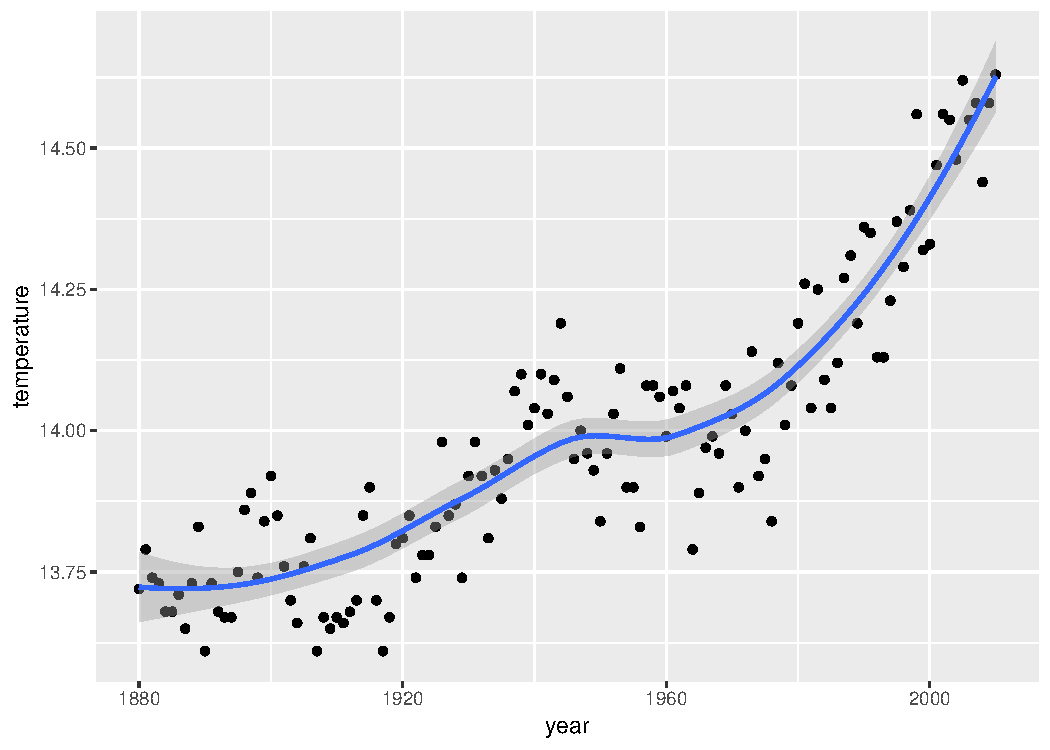
\includegraphics[width=\maxwidth]{figure/unnamed-chunk-15-1} 

\end{knitrout}
  
\end{frame}

\begin{frame}[fragile]{Cross-validation}
  
  \begin{itemize}
  \item So far, have predicted group membership from same data used to
    form the groups --- dishonest!
  \item Better: \emph{cross-validation}: form groups from all
    observations \emph{except one}, then predict group membership for
    that left-out observation.
  \item No longer cheating!
  \item Illustrate with peanuts data again.
  \end{itemize}
  
\end{frame}

\begin{frame}[fragile]{Misclassifications}
  \begin{itemize}
  \item Fitting and prediction all in one go.
  
\begin{knitrout}
\definecolor{shadecolor}{rgb}{0.969, 0.969, 0.969}\color{fgcolor}\begin{kframe}
\begin{alltt}
\hlstd{peanuts.cv}\hlkwb{=}\hlkwd{lda}\hlstd{(combo}\hlopt{~}\hlstd{y}\hlopt{+}\hlstd{smk}\hlopt{+}\hlstd{w,}\hlkwc{data}\hlstd{=peanuts,}\hlkwc{CV}\hlstd{=T)}
\hlkwd{table}\hlstd{(combo,}\hlkwc{pred}\hlstd{=peanuts.cv}\hlopt{$}\hlstd{class)}
\end{alltt}
\begin{verbatim}
##      pred
## combo 5-1 5-2 6-1 6-2 8-1 8-2
##   5-1   0   0   0   2   0   0
##   5-2   0   1   0   0   1   0
##   6-1   0   0   2   0   0   0
##   6-2   1   0   0   1   0   0
##   8-1   0   1   0   0   0   1
##   8-2   0   0   0   0   0   2
\end{verbatim}
\end{kframe}
\end{knitrout}

\item Some more misclassification this time.
  \end{itemize}

\end{frame}

\begin{frame}[fragile]{Repeat of LD plot}
 
\begin{knitrout}
\definecolor{shadecolor}{rgb}{0.969, 0.969, 0.969}\color{fgcolor}\begin{kframe}
\begin{alltt}
\hlstd{g}
\end{alltt}
\end{kframe}
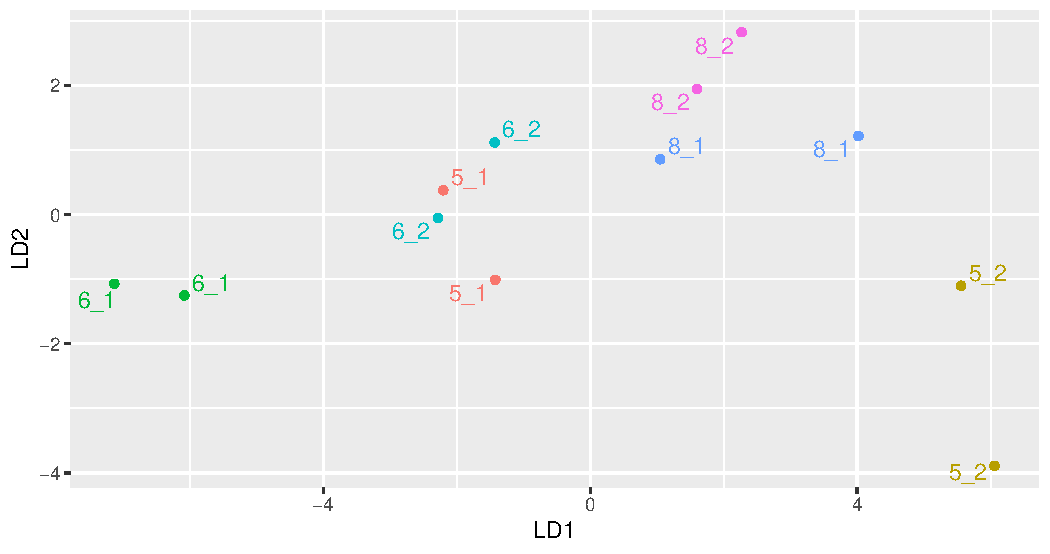
\includegraphics[width=\maxwidth]{figure/graziani-1} 

\end{knitrout}
  
\end{frame}

\begin{frame}[fragile]{Posterior probabilities}
  
\begin{knitrout}
\definecolor{shadecolor}{rgb}{0.969, 0.969, 0.969}\color{fgcolor}\begin{kframe}
\begin{alltt}
\hlstd{pp}\hlkwb{=}\hlkwd{round}\hlstd{(peanuts.cv}\hlopt{$}\hlstd{posterior,}\hlnum{3}\hlstd{)}
\hlkwd{data.frame}\hlstd{(combo,}\hlkwc{pred}\hlstd{=peanuts.cv}\hlopt{$}\hlstd{class,pp)}
\end{alltt}
\begin{verbatim}
##    combo pred  X5.1 X5.2  X6.1  X6.2  X8.1  X8.2
## 1    5-1  6-2 0.162 0.00 0.000 0.838 0.000 0.000
## 2    5-1  6-2 0.200 0.00 0.000 0.799 0.000 0.000
## 3    5-2  8-1 0.000 0.18 0.000 0.000 0.820 0.000
## 4    5-2  5-2 0.000 1.00 0.000 0.000 0.000 0.000
## 5    6-1  6-1 0.194 0.00 0.669 0.137 0.000 0.000
## 6    6-1  6-1 0.000 0.00 1.000 0.000 0.000 0.000
## 7    6-2  6-2 0.325 0.00 0.000 0.667 0.001 0.008
## 8    6-2  5-1 0.821 0.00 0.000 0.179 0.000 0.000
## 9    8-1  8-2 0.000 0.00 0.000 0.000 0.000 1.000
## 10   8-1  5-2 0.000 1.00 0.000 0.000 0.000 0.000
## 11   8-2  8-2 0.001 0.00 0.000 0.004 0.083 0.913
## 12   8-2  8-2 0.000 0.00 0.000 0.000 0.167 0.833
\end{verbatim}
\end{kframe}
\end{knitrout}
  
\end{frame}

\begin{frame}[fragile]{Why more misclassification?}
  
  \begin{itemize}
  \item When predicting group membership for one observation, only
    uses the \emph{other one} in that group.
  \item So if two in a pair are far apart, or if two groups overlap,
    great potential for misclassification.
  \item Groups \texttt{5-1} and \texttt{6-2} overlap.
  \item \texttt{5-2} closest to \texttt{8-1}s looks more like an
    \texttt{8-1} than a \texttt{5-2} (other one far away).
  \item \texttt{8-1}s relatively far apart and close to other things,
    so one appears to be a \texttt{5-2} and the other an \texttt{8-2}.
  \end{itemize}
  
\end{frame}


\begin{frame}[fragile]{Example 3: professions and leisure activities}

  \begin{itemize}
  \item 15 individuals from three different professions (politicians,
    administrators and belly dancers) each participate in four
    different leisure activities: reading, dancing, TV watching and
    skiing. After each activity they rate it on a 0--10 scale.
  \item Some of the data:

\begin{verbatim}
bellydancer 7 10 6 5
bellydancer 8 9 5 7
bellydancer 5 10 5 8
politician 5 5 5 6
politician 4 5 6 5
admin 4 2 2 5
admin 7 1 2 4
admin 6 3 3 3
\end{verbatim}
  \item How can we best use the scores on the activities to predict a person's profession?
  \item Or, what combination(s) of scores best separate data into profession groups?
  \end{itemize}

\end{frame}

\begin{frame}[fragile]{Discriminant analysis}

\begin{knitrout}
\definecolor{shadecolor}{rgb}{0.969, 0.969, 0.969}\color{fgcolor}\begin{kframe}
\begin{alltt}
\hlstd{active}\hlkwb{=}\hlkwd{read.table}\hlstd{(}\hlstr{"profile.txt"}\hlstd{,}\hlkwc{header}\hlstd{=T)}
\hlstd{active.lda}\hlkwb{=}\hlkwd{lda}\hlstd{(job}\hlopt{~}\hlstd{reading}\hlopt{+}\hlstd{dance}\hlopt{+}\hlstd{tv}\hlopt{+}\hlstd{ski,}\hlkwc{data}\hlstd{=active)}
\hlstd{active.lda}\hlopt{$}\hlstd{svd}
\end{alltt}
\begin{verbatim}
## [1] 9.856638 3.434555
\end{verbatim}
\begin{alltt}
\hlstd{active.lda}\hlopt{$}\hlstd{scaling}
\end{alltt}
\begin{verbatim}
##                 LD1        LD2
## reading -0.01297465  0.4748081
## dance   -0.95212396  0.4614976
## tv      -0.47417264 -1.2446327
## ski      0.04153684  0.2033122
\end{verbatim}
\end{kframe}
\end{knitrout}

\begin{itemize}
\item Two discriminants, first fair bit more important than second.
\item \texttt{LD1} depends (negatively) most on \texttt{dance}, a bit
  on \texttt{tv}.
\item \texttt{LD2} depends mostly on \texttt{tv}.
\end{itemize}

\end{frame}



\begin{frame}[fragile]{Misclassification}
  
\begin{knitrout}
\definecolor{shadecolor}{rgb}{0.969, 0.969, 0.969}\color{fgcolor}\begin{kframe}
\begin{alltt}
\hlstd{active.pred}\hlkwb{=}\hlkwd{predict}\hlstd{(active.lda)}
\hlkwd{table}\hlstd{(}\hlkwc{obs}\hlstd{=active}\hlopt{$}\hlstd{job,}\hlkwc{pred}\hlstd{=active.pred}\hlopt{$}\hlstd{class)}
\end{alltt}
\begin{verbatim}
##              pred
## obs           admin bellydancer politician
##   admin           5           0          0
##   bellydancer     0           5          0
##   politician      0           0          5
\end{verbatim}
\end{kframe}
\end{knitrout}

Everyone correctly classified.
  
\end{frame}

\begin{frame}[fragile]{Plotting LDs}
  
\begin{knitrout}
\definecolor{shadecolor}{rgb}{0.969, 0.969, 0.969}\color{fgcolor}\begin{kframe}
\begin{alltt}
\hlstd{mm}\hlkwb{=}\hlkwd{data.frame}\hlstd{(}\hlkwc{job}\hlstd{=active}\hlopt{$}\hlstd{job,active.pred}\hlopt{$}\hlstd{x,}\hlkwc{person}\hlstd{=}\hlnum{1}\hlopt{:}\hlnum{15}\hlstd{)}
\hlstd{g}\hlkwb{=}\hlkwd{ggplot}\hlstd{(mm,}\hlkwd{aes}\hlstd{(}\hlkwc{x}\hlstd{=LD1,}\hlkwc{y}\hlstd{=LD2,}
    \hlkwc{colour}\hlstd{=job,}\hlkwc{label}\hlstd{=job))}\hlopt{+}\hlkwd{geom_point}\hlstd{()}\hlopt{+}
    \hlkwd{geom_text_repel}\hlstd{()}\hlopt{+}\hlkwd{guides}\hlstd{(}\hlkwc{colour}\hlstd{=F) ; g}
\end{alltt}
\end{kframe}
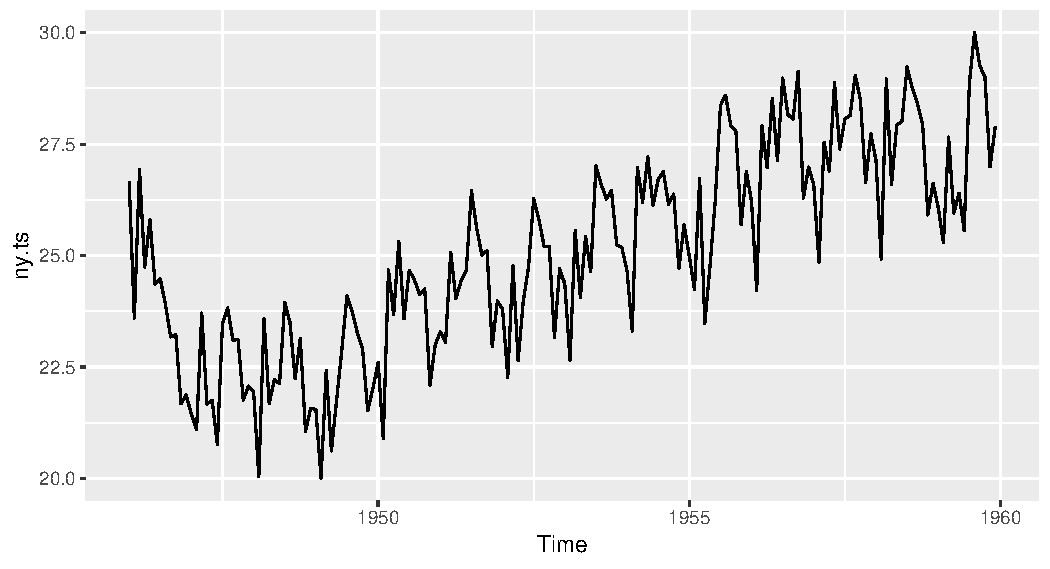
\includegraphics[width=\maxwidth]{figure/unnamed-chunk-20-1} 

\end{knitrout}
  
\end{frame}

\begin{frame}[fragile]{Comments on plot}
  
  \begin{itemize}
  \item Groups well separated: bellydancers top left, administrators
    top right, politicians lower middle.
  \item Bellydancers most negative on \texttt{LD1}: like dancing most.
  \item Administrators most positive on \texttt{LD1}: like dancing least.
  \item Politicians most negative on \texttt{LD2}: like TV-watching most.
  \end{itemize}
  
\end{frame}

\begin{frame}[fragile]{Plotting individual \texttt{person}s}
  
Make \texttt{label} be identifier of person. Now need legend:

\begin{knitrout}
\definecolor{shadecolor}{rgb}{0.969, 0.969, 0.969}\color{fgcolor}\begin{kframe}
\begin{alltt}
\hlkwd{ggplot}\hlstd{(mm,}\hlkwd{aes}\hlstd{(}\hlkwc{x}\hlstd{=LD1,}\hlkwc{y}\hlstd{=LD2,}
    \hlkwc{colour}\hlstd{=job,}\hlkwc{label}\hlstd{=person))}\hlopt{+}\hlkwd{geom_point}\hlstd{()}\hlopt{+}
    \hlkwd{geom_text_repel}\hlstd{()}
\end{alltt}
\end{kframe}
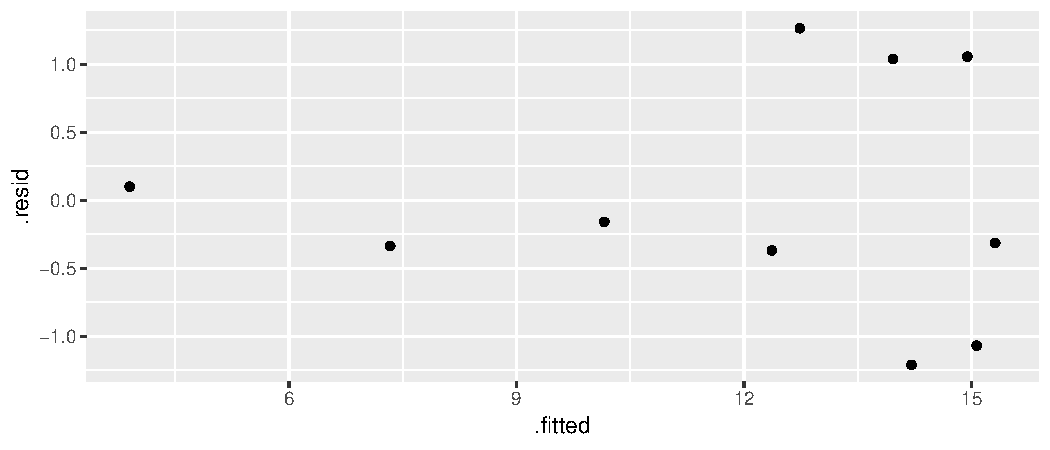
\includegraphics[width=\maxwidth]{figure/unnamed-chunk-21-1} 

\end{knitrout}
  
  
\end{frame}

\begin{frame}[fragile]{Posterior probabilities}

\begin{knitrout}\footnotesize
\definecolor{shadecolor}{rgb}{0.969, 0.969, 0.969}\color{fgcolor}\begin{kframe}
\begin{alltt}
\hlstd{pp}\hlkwb{=}\hlkwd{round}\hlstd{(active.pred}\hlopt{$}\hlstd{posterior,}\hlnum{3}\hlstd{)}
\hlkwd{data.frame}\hlstd{(}\hlkwc{obs}\hlstd{=active}\hlopt{$}\hlstd{job,}\hlkwc{pred}\hlstd{=active.pred}\hlopt{$}\hlstd{class,pp)}
\end{alltt}
\begin{verbatim}
##            obs        pred admin bellydancer politician
## 1  bellydancer bellydancer 0.000       1.000      0.000
## 2  bellydancer bellydancer 0.000       1.000      0.000
## 3  bellydancer bellydancer 0.000       1.000      0.000
## 4  bellydancer bellydancer 0.000       1.000      0.000
## 5  bellydancer bellydancer 0.000       0.997      0.003
## 6   politician  politician 0.003       0.000      0.997
## 7   politician  politician 0.000       0.000      1.000
## 8   politician  politician 0.000       0.000      1.000
## 9   politician  politician 0.000       0.002      0.998
## 10  politician  politician 0.000       0.000      1.000
## 11       admin       admin 1.000       0.000      0.000
## 12       admin       admin 1.000       0.000      0.000
## 13       admin       admin 1.000       0.000      0.000
## 14       admin       admin 1.000       0.000      0.000
## 15       admin       admin 0.982       0.000      0.018
\end{verbatim}
\end{kframe}
\end{knitrout}


Not much doubt.
\end{frame}

\begin{frame}[fragile]{Cross-validating the jobs-activities data}
  
Recall: no need for \texttt{predict}. Just pull out \texttt{class} and
make a table:  
  
\begin{knitrout}
\definecolor{shadecolor}{rgb}{0.969, 0.969, 0.969}\color{fgcolor}\begin{kframe}
\begin{alltt}
\hlstd{active.cv}\hlkwb{=}\hlkwd{lda}\hlstd{(job}\hlopt{~}\hlstd{reading}\hlopt{+}\hlstd{dance}\hlopt{+}\hlstd{tv}\hlopt{+}\hlstd{ski,}\hlkwc{data}\hlstd{=active,}\hlkwc{CV}\hlstd{=T)}
\hlkwd{table}\hlstd{(}\hlkwc{obs}\hlstd{=active}\hlopt{$}\hlstd{job,}\hlkwc{pred}\hlstd{=active.cv}\hlopt{$}\hlstd{class)}
\end{alltt}
\begin{verbatim}
##              pred
## obs           admin bellydancer politician
##   admin           5           0          0
##   bellydancer     0           4          1
##   politician      0           0          5
\end{verbatim}
\end{kframe}
\end{knitrout}

This time one of the bellydancers was classified as a politician.
  
\end{frame}

\begin{frame}[fragile]{and look at the posterior probabilities}
  
picking out the ones where things are not certain:

\begin{knitrout}\footnotesize
\definecolor{shadecolor}{rgb}{0.969, 0.969, 0.969}\color{fgcolor}\begin{kframe}
\begin{alltt}
\hlstd{pp}\hlkwb{=}\hlkwd{round}\hlstd{(active.cv}\hlopt{$}\hlstd{posterior,}\hlnum{3}\hlstd{)}
\hlkwd{data.frame}\hlstd{(}\hlkwc{obs}\hlstd{=active}\hlopt{$}\hlstd{job,}\hlkwc{pred}\hlstd{=active.cv}\hlopt{$}\hlstd{class,pp)} \hlopt
  \hlkwd{mutate}\hlstd{(}\hlkwc{max}\hlstd{=}\hlkwd{pmax}\hlstd{(admin,bellydancer,politician))} \hlopt
  \hlkwd{filter}\hlstd{(max}\hlopt{<}\hlnum{0.9995}\hlstd{)}
\end{alltt}
\begin{verbatim}
##           obs       pred admin bellydancer politician   max
## 1 bellydancer politician 0.000       0.001      0.999 0.999
## 2  politician politician 0.006       0.000      0.994 0.994
## 3  politician politician 0.001       0.000      0.999 0.999
## 4  politician politician 0.000       0.009      0.991 0.991
## 5       admin      admin 0.819       0.000      0.181 0.819
\end{verbatim}
\end{kframe}
\end{knitrout}
%$
\begin{itemize}
\item Bellydancer was ``definitely'' a politician!
\item One of the administrators might have been a politician too.
\end{itemize}
  
\end{frame}


\begin{frame}[fragile]{Why did things get misclassified?}

  \begin{minipage}[t]{0.7\linewidth}
\begin{knitrout}
\definecolor{shadecolor}{rgb}{0.969, 0.969, 0.969}\color{fgcolor}\begin{kframe}
\begin{alltt}
\hlstd{g}
\end{alltt}
\end{kframe}
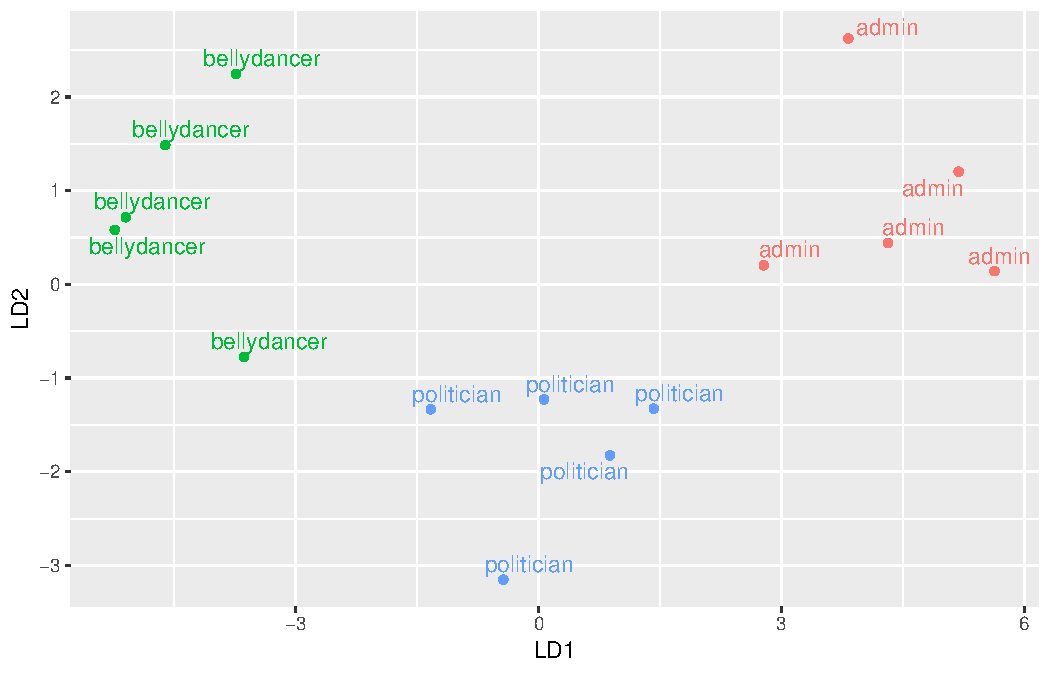
\includegraphics[width=\maxwidth]{figure/nesta-1} 

\end{knitrout}
  \end{minipage}
  \begin{minipage}[t]{0.28\linewidth}
    \begin{itemize}
    \item Go back to plot of \texttt{active.lda}:
    \item one bellydancer much closer to the politicians,
    \item one administrator a bit closer to the politicians.
    \end{itemize}
  \end{minipage}
  
  

  
\end{frame}


\begin{frame}[fragile]{Example 4: remote-sensing data}

  \begin{itemize}
  \item View 38 crops from air, measure 4 variables \verb=x1-x4=.
  \item Go back and record what each crop was.
  \item Can we use the 4 variables to distinguish crops?
  \end{itemize}
\end{frame}

\begin{frame}[fragile]{Starting off: number of LDs}
  
\begin{knitrout}
\definecolor{shadecolor}{rgb}{0.969, 0.969, 0.969}\color{fgcolor}\begin{kframe}
\begin{alltt}
\hlstd{crops}\hlkwb{=}\hlkwd{read.table}\hlstd{(}\hlstr{"remote-sensing.txt"}\hlstd{,}\hlkwc{header}\hlstd{=T)}
\hlkwd{attach}\hlstd{(crops)}
\hlstd{crops.lda}\hlkwb{=}\hlkwd{lda}\hlstd{(crop}\hlopt{~}\hlstd{x1}\hlopt{+}\hlstd{x2}\hlopt{+}\hlstd{x3}\hlopt{+}\hlstd{x4)}
\hlstd{crops.lda}\hlopt{$}\hlstd{svd}
\end{alltt}
\begin{verbatim}
## [1] 2.2858251 1.1866352 0.6394041 0.2303634
\end{verbatim}
\end{kframe}
\end{knitrout}

\begin{itemize}
\item 4 LDs (four variables, six groups).
\item 1st one important, maybe 2nd as well.
\end{itemize}
  
\end{frame}


\begin{frame}[fragile]{Connecting original variables and LDs}
  
\begin{knitrout}
\definecolor{shadecolor}{rgb}{0.969, 0.969, 0.969}\color{fgcolor}\begin{kframe}
\begin{alltt}
\hlstd{crops.lda}\hlopt{$}\hlstd{means}
\end{alltt}
\begin{verbatim}
##                  x1       x2       x3       x4
## Clover     46.36364 32.63636 34.18182 36.63636
## Corn       15.28571 22.71429 27.42857 33.14286
## Cotton     34.50000 32.66667 35.00000 39.16667
## Soybeans   21.00000 27.00000 23.50000 29.66667
## Sugarbeets 31.00000 32.16667 20.00000 40.50000
\end{verbatim}
\begin{alltt}
\hlkwd{round}\hlstd{(crops.lda}\hlopt{$}\hlstd{scaling,}\hlnum{3}\hlstd{)}
\end{alltt}
\begin{verbatim}
##       LD1    LD2    LD3    LD4
## x1 -0.061  0.009 -0.030 -0.015
## x2 -0.025  0.043  0.046  0.055
## x3  0.016 -0.079  0.020  0.009
## x4  0.000 -0.014  0.054 -0.026
\end{verbatim}
\end{kframe}
\end{knitrout}

\begin{itemize}
\item Links groups to original variables to LDs.
\end{itemize}
\end{frame}

\begin{frame}[fragile]{\texttt{LD1} and \texttt{LD2}}
  
\begin{knitrout}
\definecolor{shadecolor}{rgb}{0.969, 0.969, 0.969}\color{fgcolor}\begin{kframe}
\begin{alltt}
\hlkwd{round}\hlstd{(crops.lda}\hlopt{$}\hlstd{scaling,}\hlnum{3}\hlstd{)}
\end{alltt}
\begin{verbatim}
##       LD1    LD2    LD3    LD4
## x1 -0.061  0.009 -0.030 -0.015
## x2 -0.025  0.043  0.046  0.055
## x3  0.016 -0.079  0.020  0.009
## x4  0.000 -0.014  0.054 -0.026
\end{verbatim}
\end{kframe}
\end{knitrout}
%$
\begin{itemize}
\item \texttt{LD1} mostly \texttt{x1} (minus), so clover low on
  \texttt{LD1}, corn high.
\item \texttt{LD2} \texttt{x3} (minus), \texttt{x2} (plus), so
  sugarbeets should be high on \texttt{LD2}.
\end{itemize}

  
\end{frame}

\begin{frame}[fragile]{Predictions}
  
  \begin{itemize}
  \item Thus:
\begin{knitrout}
\definecolor{shadecolor}{rgb}{0.969, 0.969, 0.969}\color{fgcolor}\begin{kframe}
\begin{alltt}
\hlstd{crops.pred}\hlkwb{=}\hlkwd{predict}\hlstd{(crops.lda)}
\hlkwd{table}\hlstd{(}\hlkwc{obs}\hlstd{=crops}\hlopt{$}\hlstd{crop,}\hlkwc{pred}\hlstd{=crops.pred}\hlopt{$}\hlstd{class)}
\end{alltt}
\begin{verbatim}
##             pred
## obs          Clover Corn Cotton Soybeans Sugarbeets
##   Clover          6    0      3        0          2
##   Corn            0    6      0        1          0
##   Cotton          3    0      1        2          0
##   Soybeans        0    1      1        3          1
##   Sugarbeets      1    1      0        2          2
\end{verbatim}
\end{kframe}
\end{knitrout}
\item Not very good, eg.\ only 6 of 11 \texttt{Clover} classified correctly.
\item Set up for plot:
  
\begin{knitrout}
\definecolor{shadecolor}{rgb}{0.969, 0.969, 0.969}\color{fgcolor}\begin{kframe}
\begin{alltt}
\hlstd{mm}\hlkwb{=}\hlkwd{data.frame}\hlstd{(}\hlkwc{crop}\hlstd{=crops}\hlopt{$}\hlstd{crop,crops.pred}\hlopt{$}\hlstd{x)}
\end{alltt}
\end{kframe}
\end{knitrout}
    
  \end{itemize}

  
\end{frame}


\begin{frame}[fragile]{Plotting the LDs}
  
\begin{knitrout}
\definecolor{shadecolor}{rgb}{0.969, 0.969, 0.969}\color{fgcolor}\begin{kframe}
\begin{alltt}
\hlkwd{ggplot}\hlstd{(mm,}\hlkwd{aes}\hlstd{(}\hlkwc{x}\hlstd{=LD1,}\hlkwc{y}\hlstd{=LD2,}\hlkwc{colour}\hlstd{=crop,}\hlkwc{label}\hlstd{=crop))}\hlopt{+}
  \hlkwd{geom_point}\hlstd{()}\hlopt{+}\hlkwd{geom_text_repel}\hlstd{()}\hlopt{+}
  \hlkwd{guides}\hlstd{(}\hlkwc{colour}\hlstd{=F)}
\end{alltt}
\end{kframe}
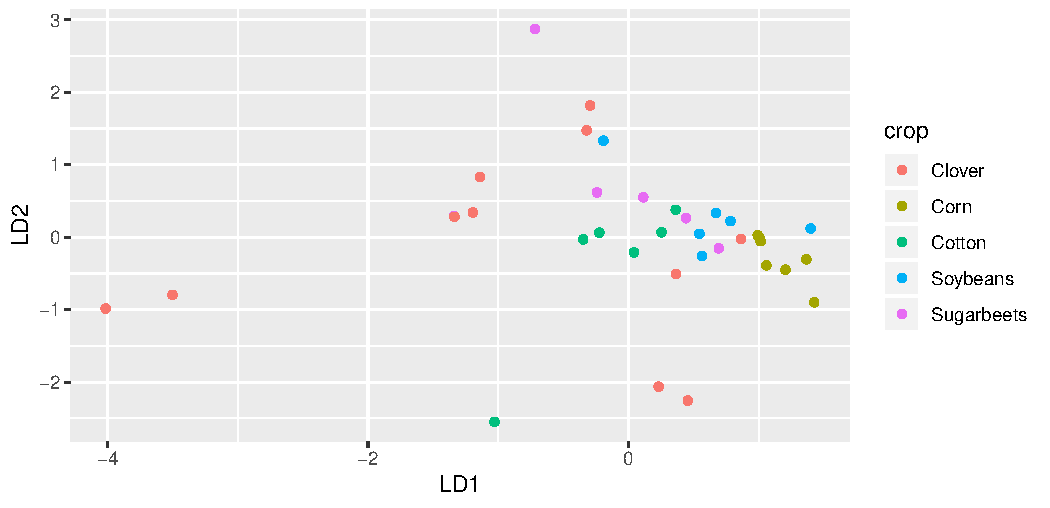
\includegraphics[width=\maxwidth]{figure/piacentini-1} 

\end{knitrout}
  
\end{frame}

\begin{frame}[figure]{Comments}
  
  \begin{itemize}
  \item Corn high on LD1 (right).
  \item Clover all over the place, but mostly low on LD1 (left).
  \item Sugarbeets tend to be high on LD2.
  \item Cotton tends to be low on LD2.
  \item Very mixed up.
  \end{itemize}
  
\end{frame}

\begin{frame}[fragile]{Try removing Clover}

  \begin{itemize}

  \item the \texttt{dplyr} way:
    
\begin{knitrout}
\definecolor{shadecolor}{rgb}{0.969, 0.969, 0.969}\color{fgcolor}\begin{kframe}
\begin{alltt}
\hlstd{crops} \hlopt \hlkwd{filter}\hlstd{(crop}\hlopt{!=}\hlstr{"Clover"}\hlstd{)} \hlkwb{->} \hlstd{crops2}
\hlstd{crops2.lda}\hlkwb{=}\hlkwd{lda}\hlstd{(crop}\hlopt{~}\hlstd{x1}\hlopt{+}\hlstd{x2}\hlopt{+}\hlstd{x3}\hlopt{+}\hlstd{x4,}\hlkwc{data}\hlstd{=crops2)}
\end{alltt}


{\ttfamily\noindent\color{warningcolor}{\#\# Warning in lda.default(x, grouping, ...): group Clover is empty}}\end{kframe}
\end{knitrout}

\item LDs for \texttt{crops2} will be different from before.
\item Concentrate on plot and posterior probs.

\begin{knitrout}
\definecolor{shadecolor}{rgb}{0.969, 0.969, 0.969}\color{fgcolor}\begin{kframe}
\begin{alltt}
\hlstd{crops2.pred}\hlkwb{=}\hlkwd{predict}\hlstd{(crops2.lda)}
\hlstd{mm}\hlkwb{=}\hlkwd{data.frame}\hlstd{(}\hlkwc{crop}\hlstd{=crops2}\hlopt{$}\hlstd{crop,crops2.pred}\hlopt{$}\hlstd{x)}
\end{alltt}
\end{kframe}
\end{knitrout}
  
\end{itemize}
  
\end{frame}

\begin{frame}[fragile]{\texttt{lda} output}
  
  
Different from before:

\begin{knitrout}\footnotesize
\definecolor{shadecolor}{rgb}{0.969, 0.969, 0.969}\color{fgcolor}\begin{kframe}
\begin{alltt}
\hlstd{crops2.lda}\hlopt{$}\hlstd{means}
\end{alltt}
\begin{verbatim}
##                  x1       x2       x3       x4
## Corn       15.28571 22.71429 27.42857 33.14286
## Cotton     34.50000 32.66667 35.00000 39.16667
## Soybeans   21.00000 27.00000 23.50000 29.66667
## Sugarbeets 31.00000 32.16667 20.00000 40.50000
\end{verbatim}
\begin{alltt}
\hlstd{crops2.lda}\hlopt{$}\hlstd{svd}
\end{alltt}
\begin{verbatim}
## [1] 3.3639389 1.6054750 0.4180292
\end{verbatim}
\begin{alltt}
\hlstd{crops2.lda}\hlopt{$}\hlstd{scaling}
\end{alltt}
\begin{verbatim}
##            LD1          LD2           LD3
## x1  0.14077479  0.007780184 -0.0312610362
## x2  0.03006972  0.007318386  0.0085401510
## x3 -0.06363974 -0.099520895 -0.0005309869
## x4 -0.00677414 -0.035612707  0.0577718649
\end{verbatim}
\end{kframe}
\end{knitrout}
  
\end{frame}

\begin{frame}[fragile]{Plot}

A bit more clustered:
  
\begin{knitrout}
\definecolor{shadecolor}{rgb}{0.969, 0.969, 0.969}\color{fgcolor}\begin{kframe}
\begin{alltt}
\hlkwd{ggplot}\hlstd{(mm,}\hlkwd{aes}\hlstd{(}\hlkwc{x}\hlstd{=LD1,}\hlkwc{y}\hlstd{=LD2,}\hlkwc{label}\hlstd{=crop,}\hlkwc{colour}\hlstd{=crop))}\hlopt{+}
  \hlkwd{geom_point}\hlstd{()}\hlopt{+}\hlkwd{geom_text_repel}\hlstd{()}\hlopt{+}\hlkwd{guides}\hlstd{(}\hlkwc{colour}\hlstd{=F)}
\end{alltt}
\end{kframe}
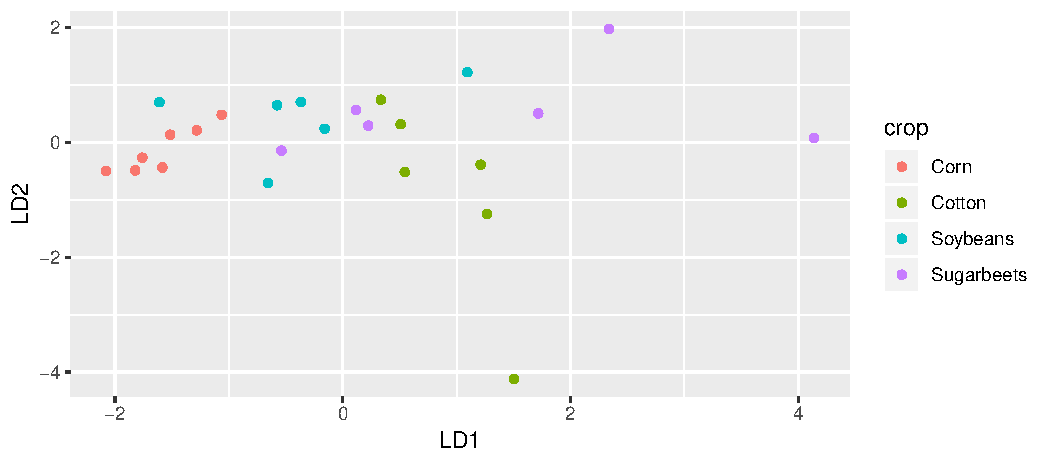
\includegraphics[width=\maxwidth]{figure/nedved-1} 

\end{knitrout}

\end{frame}

\begin{frame}[fragile]{Quality of classification}
  
\begin{knitrout}
\definecolor{shadecolor}{rgb}{0.969, 0.969, 0.969}\color{fgcolor}\begin{kframe}
\begin{alltt}
\hlkwd{table}\hlstd{(}\hlkwc{obs}\hlstd{=crops2}\hlopt{$}\hlstd{crop,}\hlkwc{pred}\hlstd{=crops2.pred}\hlopt{$}\hlstd{class)}
\end{alltt}
\begin{verbatim}
##             pred
## obs          Clover Corn Cotton Soybeans Sugarbeets
##   Clover          0    0      0        0          0
##   Corn            0    6      0        1          0
##   Cotton          0    0      4        2          0
##   Soybeans        0    2      0        3          1
##   Sugarbeets      0    0      0        3          3
\end{verbatim}
\end{kframe}
\end{knitrout}

Better.
  
\end{frame}

\begin{frame}[fragile]{Posterior probs, the wrong ones}
 

  
  
{\footnotesize  
\begin{knitrout}
\definecolor{shadecolor}{rgb}{0.969, 0.969, 0.969}\color{fgcolor}\begin{kframe}
\begin{alltt}
\hlstd{post}\hlkwb{=}\hlkwd{round}\hlstd{(crops2.pred}\hlopt{$}\hlstd{posterior,}\hlnum{3}\hlstd{)}
\hlkwd{data.frame}\hlstd{(}\hlkwc{obs}\hlstd{=crops2}\hlopt{$}\hlstd{crop,}\hlkwc{pred}\hlstd{=crops2.pred}\hlopt{$}\hlstd{class,post)} \hlopt
  \hlkwd{filter}\hlstd{(obs}\hlopt{!=}\hlstd{pred)}
\end{alltt}
\begin{verbatim}
##          obs       pred  Corn Cotton Soybeans Sugarbeets
## 1       Corn   Soybeans 0.443  0.034    0.494      0.029
## 2   Soybeans Sugarbeets 0.010  0.107    0.299      0.584
## 3   Soybeans       Corn 0.684  0.009    0.296      0.011
## 4   Soybeans       Corn 0.467  0.199    0.287      0.047
## 5     Cotton   Soybeans 0.056  0.241    0.379      0.324
## 6     Cotton   Soybeans 0.066  0.138    0.489      0.306
## 7 Sugarbeets   Soybeans 0.381  0.146    0.395      0.078
## 8 Sugarbeets   Soybeans 0.106  0.144    0.518      0.232
## 9 Sugarbeets   Soybeans 0.088  0.207    0.489      0.216
\end{verbatim}
\end{kframe}
\end{knitrout}
}

\begin{itemize}
\item These were the misclassified ones, but the posterior probability
  of being correct was not usually too low.
\item The correctly-classified ones are not very clear-cut either.

\end{itemize}
  
\end{frame}

\begin{frame}[fragile]{Manova}
  
Began discriminant analysis as a followup to MANOVA. Do our variables
significantly separate the crops (excluding Clover)?

\begin{knitrout}
\definecolor{shadecolor}{rgb}{0.969, 0.969, 0.969}\color{fgcolor}\begin{kframe}
\begin{alltt}
\hlstd{response}\hlkwb{=}\hlkwd{with}\hlstd{(crops2,}\hlkwd{cbind}\hlstd{(x1,x2,x3,x4))}
\hlstd{crops2.manova}\hlkwb{=}\hlkwd{manova}\hlstd{(response}\hlopt{~}\hlstd{crop,}\hlkwc{data}\hlstd{=crops2)}
\hlkwd{summary}\hlstd{(crops2.manova)}
\end{alltt}
\begin{verbatim}
##           Df Pillai approx F num Df den Df  Pr(>F)  
## crop       3 0.9113   2.1815     12     60 0.02416 *
## Residuals 21                                        
## ---
## Signif. codes:  
## 0 '***' 0.001 '**' 0.01 '*' 0.05 '.' 0.1 ' ' 1
\end{verbatim}
\end{kframe}
\end{knitrout}

Yes, at least one of the crops differs (in means) from the others. So
it is worth doing this analysis.

We did this the wrong way around, though!
  
\end{frame}

\begin{frame}[fragile]{The right way around}
  
  \begin{itemize}
  \item \emph{First}, do a MANOVA to see whether any of the groups
    differ significantly on any of the variables.
  \item \emph{If the MANOVA is significant}, do a discriminant
    analysis in the hopes of understanding how the groups are different.
  \item For remote-sensing data (without Clover):
    \begin{itemize}
    \item LD1 a fair bit more important than LD2 (definitely ignore LD3).
    \item LD1 depends mostly on \texttt{x1}, on which Cotton was high
      and Corn was low. 
    \end{itemize}

  \item Discriminant analysis in MANOVA plays the same kind of role
    that Tukey does in ANOVA.
  \end{itemize}
  
\end{frame}





